Now, we elaborate on how we trap actual neutral atoms in our tweezer array. 
The optical dipole traps are in the order of mK deep and thus need to be loaded with cold atoms from a magneto-optical trap. 
The construction of the vacuum and atom source of the magneto-optical trap are elaborated upon in \cref{sec:VacuumAtom}.
The laser system used for the MOT is explained in \cref{sec:LaserSystem} and fluorescence images from the MOT are shown in \cref{sec:MOTresult}.
We finish up on how to load atoms from our MOT in the tweezer array and image them in \cref{sec:Tweezers}.

\section{Vacuum and Atom Source}\label{sec:VacuumAtom}

A sketch of the most important components in the vacuum design is shown in \cref{fig:VacuumSetup}.
The core of the experiment is the glass cell.
The glass cell has $120\times30\times30$ mm outer dimensions and is optically contacted\footnote{The glass cell was provided to us by our collaborators from the University of Amsterdam.}.
The microscope objective is placed in the vertical direction: this setup was designed with using it for Sr in mind.
When working with Sr, atoms are typically loaded from the hotter blue MOT into the much colder red MOT (see \cref{subsec:Transitions}).
Because the scattering force for the red MOT is much weaker as a result of the narrow-linewidth, gravity starts to play a role and the atoms in the MOT sags to a flatter shape. 
Therefore, the tweezer array for Sr should be produced in the horizontal plane. 

The coils producing the magnetic field gradient should also be placed near the cell. 
To still have room for all 6 MOT beams, two MOT beams and their retro-reflection pass the cell under a 60 degree vertical angle, leaving room for the microscope objective. 
The last MOT beam is sent through the center hole of the anti-Helmholtz magnetic field coils.
To allow for placement of optics in the vertical direction, a vertical breadboard was used. 
In \cref{fig:VacuumSetup} the vertical breadboard is shown along with the vertical MOT beams and the magnetic field coils. 
Also the microscope objective is shown on the bottom of the cell.
The center of the glass cell is positioned 110 mm away from the vertical breadboard and 300 mm from the optical table. 
The housing for the magnetic field coils was designed by Deon Janse van Rensburg and Rik van Herk and is shown in \cref{fig:Coils} in \cref{sec:TweezerImaging}.

A real life picture of the glass cell is shown in \cref{fig:Chamber}.
To minimize collisions with the background gas and improve the lifetime of the MOT and atoms in optical tweezers, it is pumped down to ultra-high vacuum. 
To pump the cell down, the glass cell is connected to a vacuum chamber (\cref{fig:VacuumSetup}, left).
To allow for more room around the glass cell, in between the vacuum vessel and the glass cell an extension tube is added.
We attach a turbomolecular pump to the chamber using a valve (not shown in the figure) and pump down to $\sim 10^{-8}$ mbar.
This pressure was measured using a pressure Gauge (\cref{fig:Chamber}).
To reach a better vacuum, the system was baked for a duration of two weeks at 130${}^{\circ}$C by Rik van Herk \cite{Herk2022}.

As atom source, a set of Rb dispensers\footnote{SAES Getters Alkali Metal Dispensers.} is used.
Only one dispenser is connected at a time, but we installed a triplet for redundancy.
The amount of Rb released can be controlled by the current running through the dispensers.
We typically run the dispensers at $\sim$ 5A.
The dispensers are mounted to the vacuum chamber using a CF40 flange.
We first ran the dispensers for 30 minutes while leaving the turbo pump on to get rid of the oxidation layer on the dispenser.
Next, we activate the non-evaporative getter\footnote{NEXTorr Z 100 NEG - ion combination pump.} by heating it to 500${}^{\circ}$C while pumping away its out gassing using the turbo pump. 
Finally, after closing the turbo valve and turning on the ion pump we reached a pressure of $\sim 2\times 10^{-10}$ mbar, as measured using the ion pump (the pressure gauge is not usable in this pressure regime).
When turning on the dispensers, the pressure temporarily jumps the $10^{-9}$ mbar levels, quickly returning to $10^{-10}$ when turning them off again. 


\begin{figure}
	\begin{subfigure}{.5\linewidth}
		\flushleft
		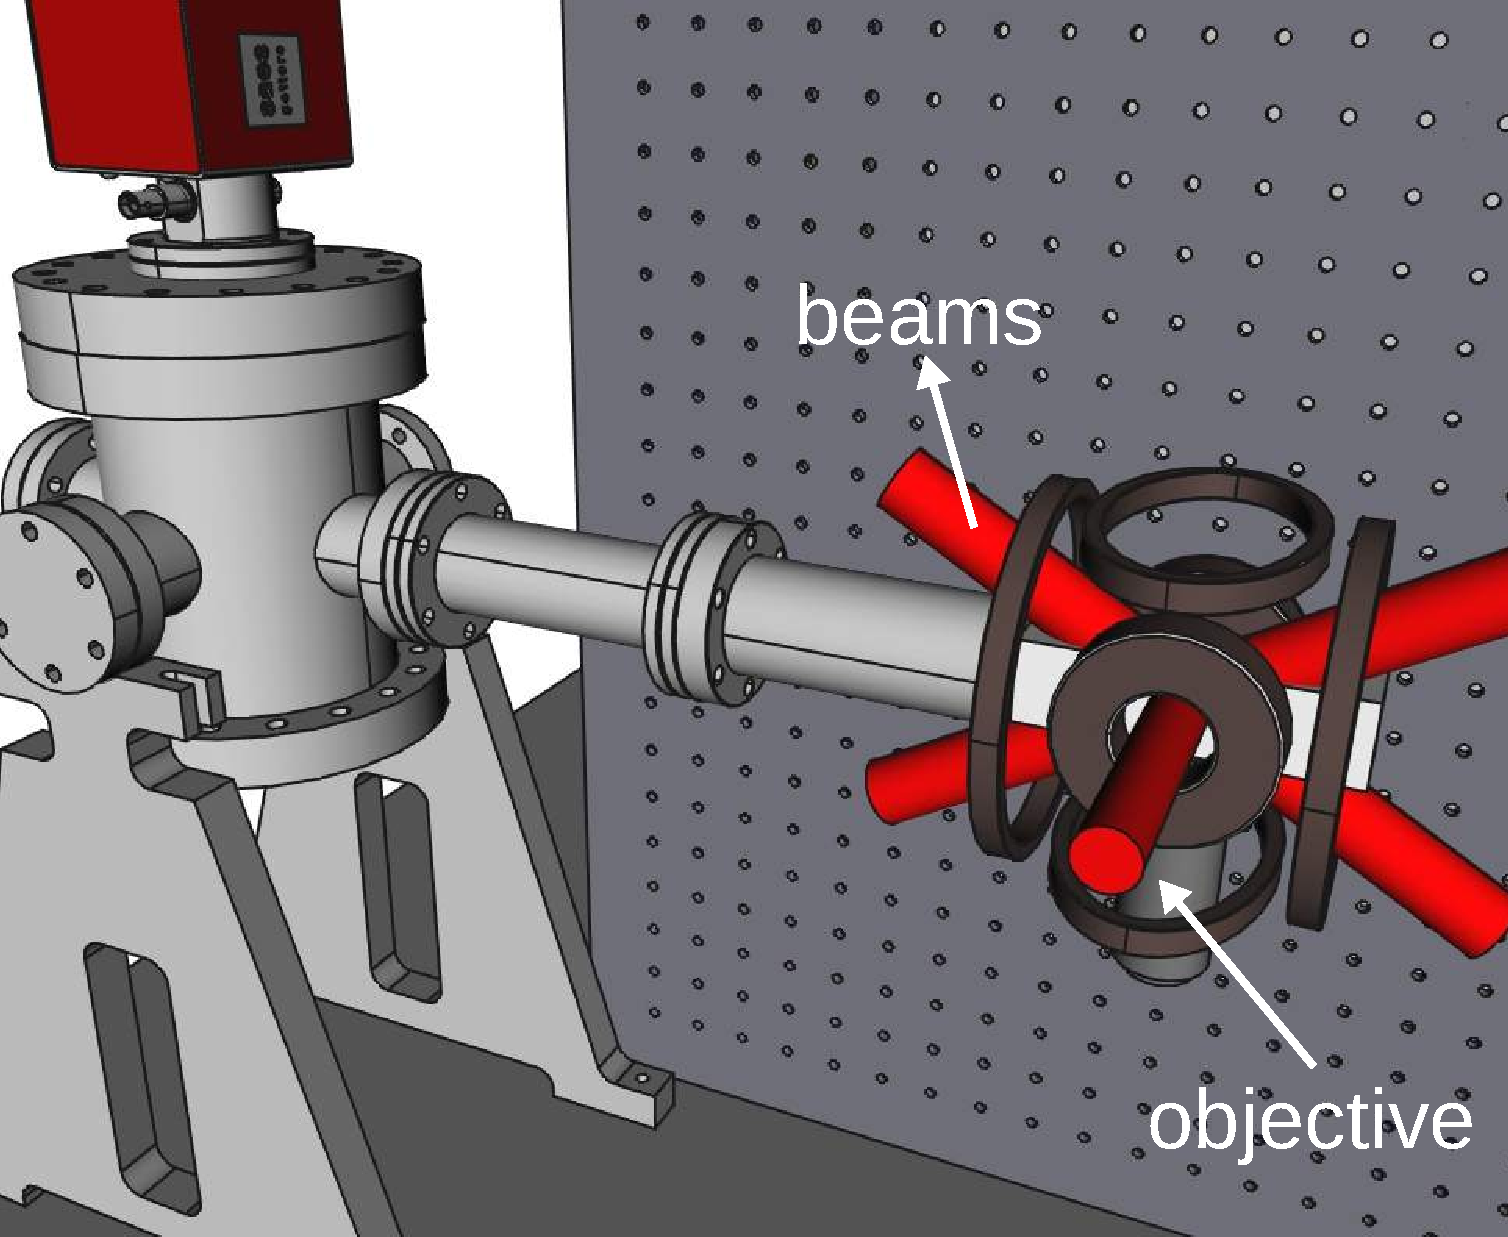
\includegraphics[height=6.5cm]{figures/CADeditSmall.pdf}
		\caption{}
		\label{fig:VacuumSetup}
	\end{subfigure}
	\hfill
	\begin{subfigure}{.49\linewidth}
		\flushright
		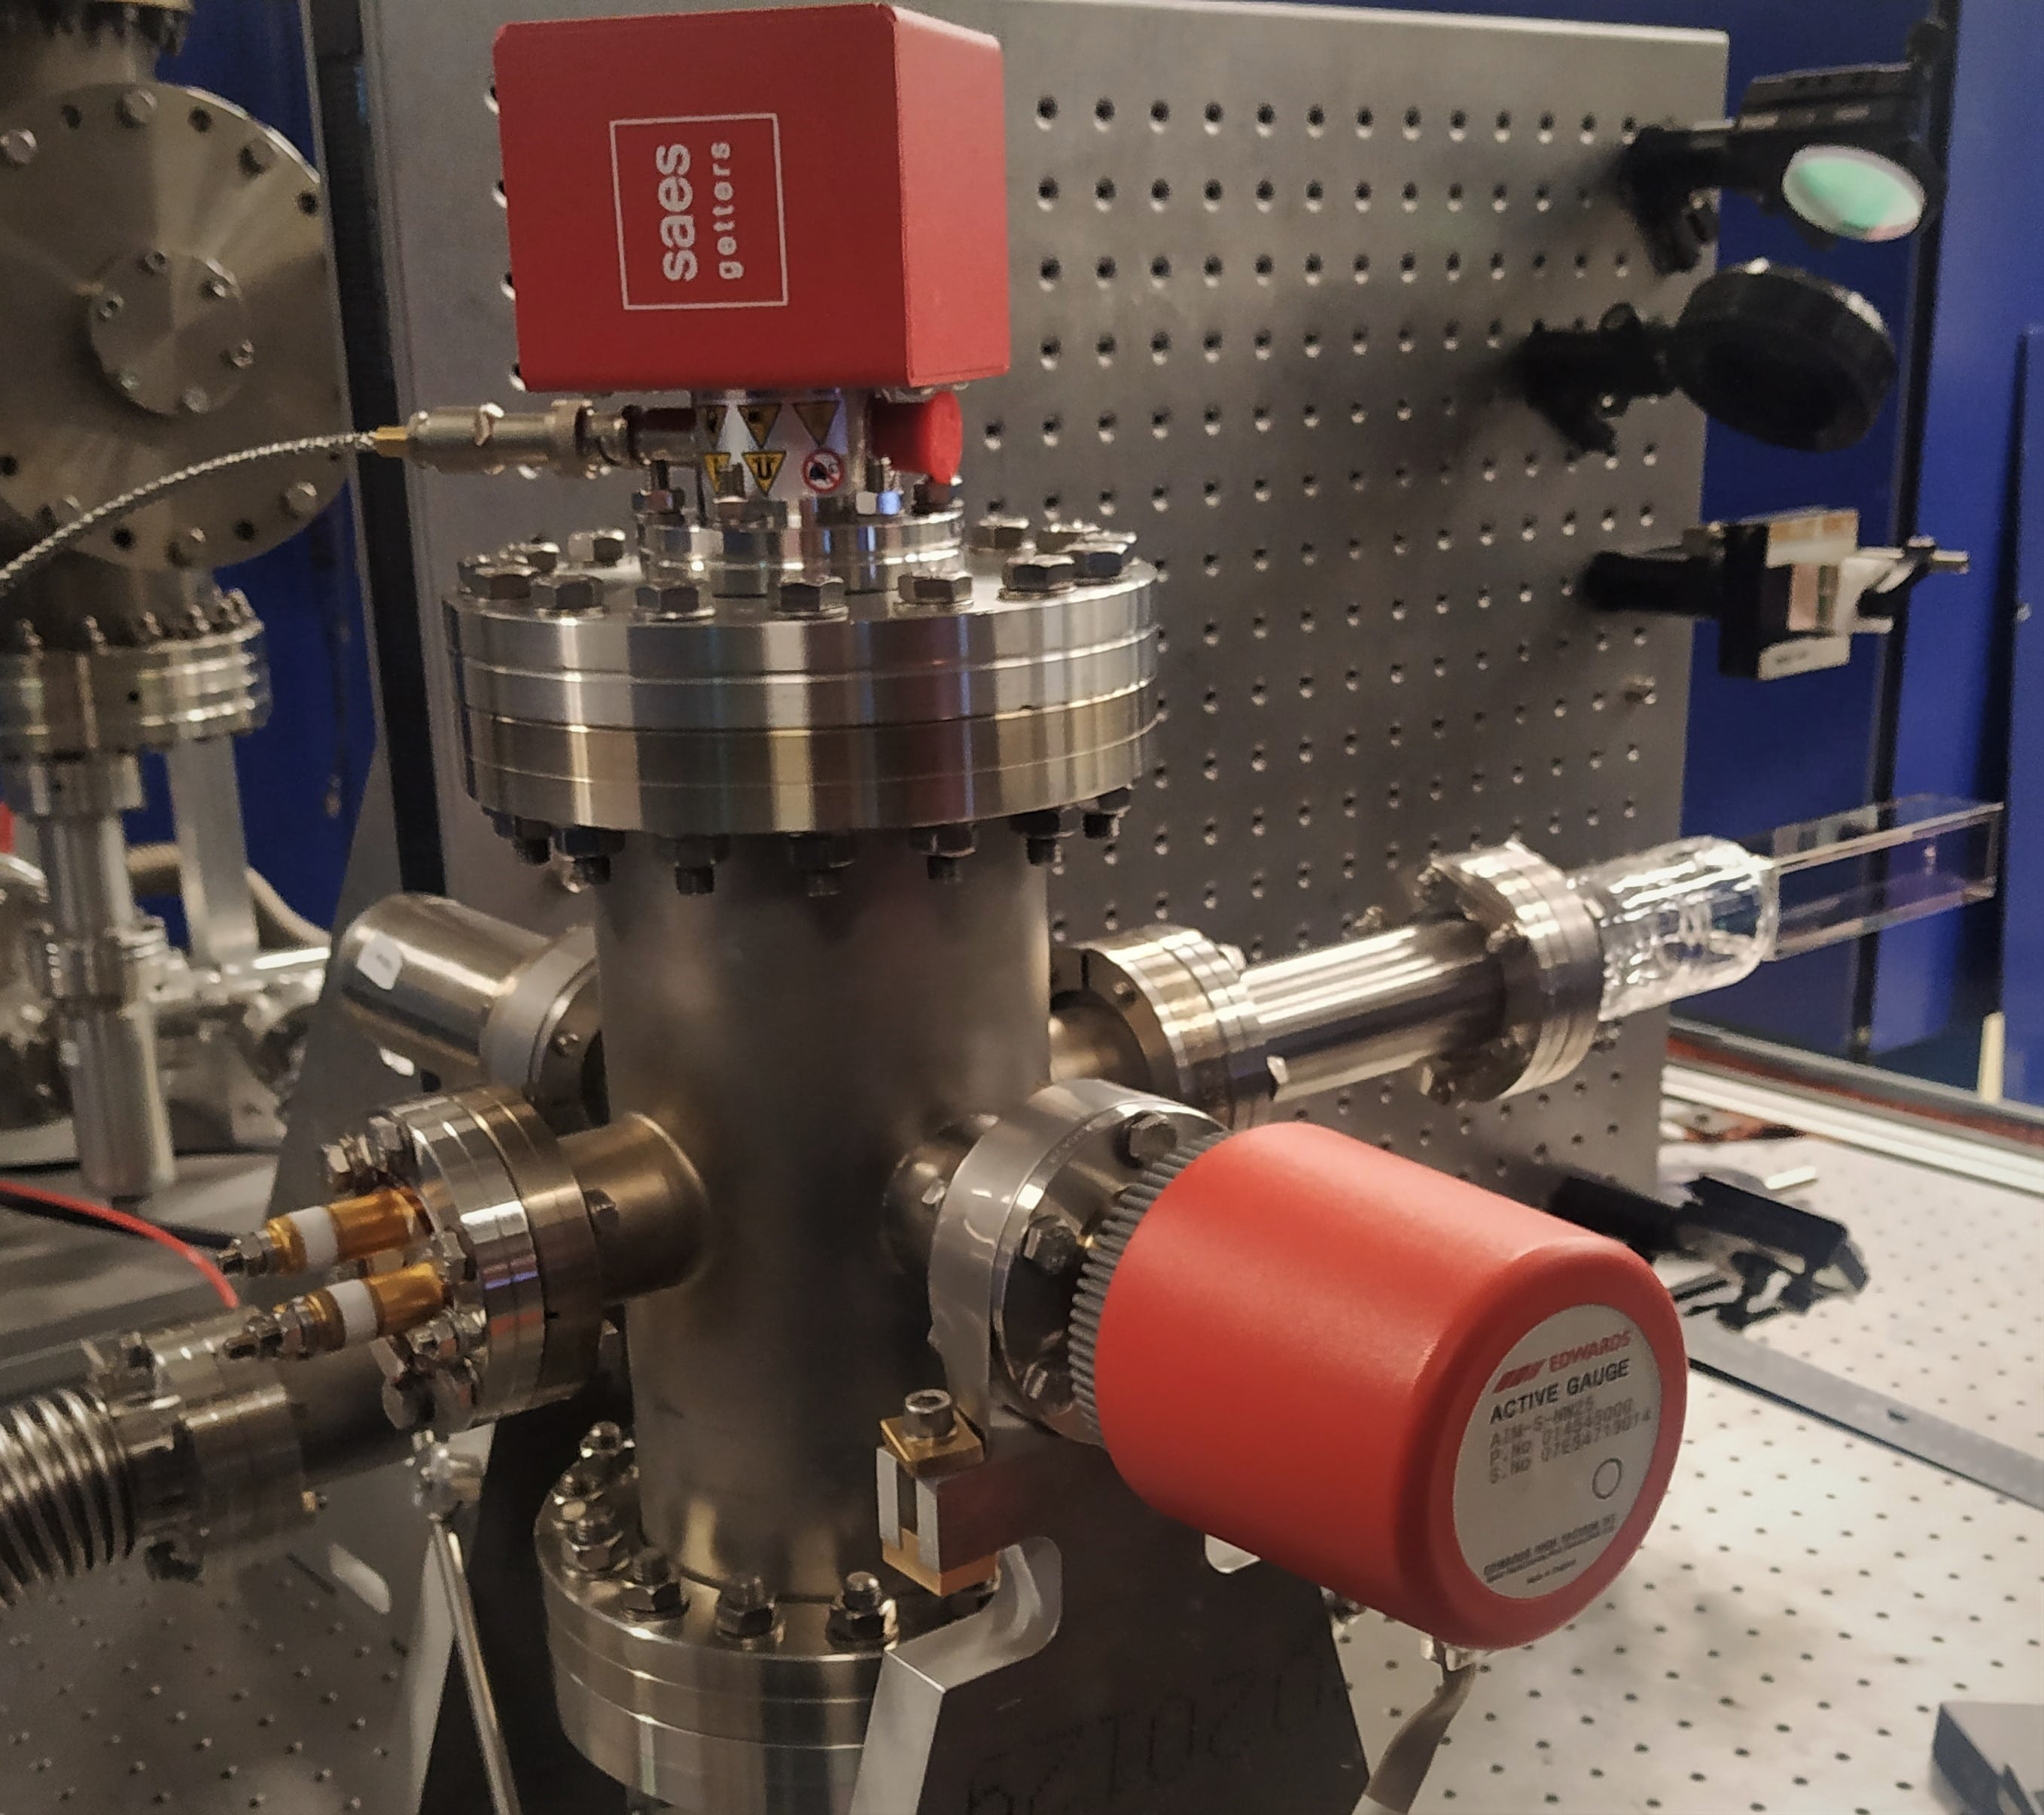
\includegraphics[height=6.5cm]{figures/Chamber.jpg}
		\caption{}
		\label{fig:Chamber}
	\end{subfigure}
	\caption{\textsf{\textbf{a)}} CAD drawing of the vacuum vessel connected to the glass cell on the right. 
	Around the glass cell, 4 out of 6 MOT beams are shown along with the magnetic field coils and a single microscope objective on the bottom. 
	CAD drawing by Eddy Rietman.
    \textsf{\textbf{b)}} Picture of the vacuum components: top: ion/getter pump. Right: glass cell. Also connected to the chamber from left to right: valve for turbo pump, triplet of Rb dispensers and pressure gauge.}
\end{figure}

\section{Laser System}\label{sec:LaserSystem}

For the laser system we recycled a significant part of the previous setup \cite{Reijnders2010}.
The atomic species we selected is Rb-85 because it is the most abundant isotope. 
A Rb-85 MOT requires two lasers: a trapping/cooling laser as well as a repump laser to recycle back atoms that end up in the wrong ground state (\cref{sec:PracticeRb}).

For the laser cooling and trapping beams we used a Toptica DLX110 diode laser. This laser should be able to produce $\sim 1$ W of power, but in current condition we typically output $\sim 500$ mW, which is already plenty of power for what we need. 
\begin{figure}[t]
    \centering
    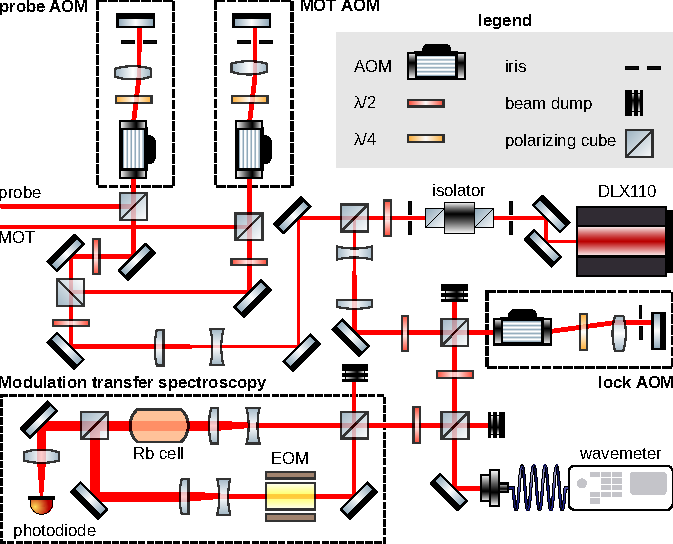
\includegraphics[width=\linewidth]{figures/RbLaserSetup.pdf}
    \caption{Laser system for the trapping and repump laser system for \textsuperscript{85}Rb \cite{Reijnders2010}.
    A section of laser light is split off to the modulation transfer spectroscopy (bottom left), after first double passing the lock \ac{AOM} (right). 
    Top: set of AOMs for the MOT and probe light.
    }
    \label{fig:RbLaserSetup}
\end{figure}
The laser is shown in \cref{fig:RbLaserSetup}.
The laser frequency is stabilized using the modulation transfer spectroscopy method \cite{Reijnders2010,McCarron2008}.
A fraction of power is split off to the section where this method is implemented  (bottom-left, \cref{fig:RbLaserSetup}) after being offset-locked using the lock \ac{AOM} (right) set to $84.5$ MHz\footnote{All frequencies are angular and have an additional $2\pi$ pre-factor.}.
The majority of power is set to the MOT (glass cell) after first passing the MOT AOM (\cref{fig:RbLaserSetup}, top).
This AOM is set to 80 MHz, which is $2 \times (80 - 84.5) = -9$ MHz from the resonance frequency, which is roughly equivalent to a detuning of $\delta = -1.5 \gamma$.
We typically use about $80$ mW of power for the MOT beams as measured after the \ac{AOM} in \cref{fig:RbLaserSetup}.
We have another AOM, which we use to make probe light, the light to induce fluorescence of the atoms when they are trapped in the optical tweezers.
This is explained in \cref{sec:TweezerImaging}.

\begin{figure}[t]
    \centering
    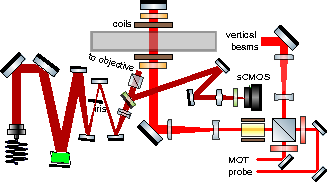
\includegraphics[width=\textwidth]{figures/MOTupview.pdf}
    \caption{
    Top view on the glass cell.
    The MOT laser beam is split into a horizontal beam, traveling through the anti-Helmholtz coils, as well as a part which will be split in the vertically angled beams (see \cref{fig:GlassCellSide}). 
    Probe light is mixed in the horizontal beam path using the same polarizing cube. 
    Both sections are expanded using a beam expander.
    This horizontal beam also contains the repump light using the \ac{EOM}.
    Furthermore the tweezer beam sent to the objective is shown, as well as the fluorescence separated from it using the \acf{DM}.
    The tweezer beam is shown under a slight angle here with respect to the horizontal MOT beam for better visibility. 
    }
    \label{fig:GlassCellTop}
\end{figure}

Apart from the main cooling and trapping laser, a repump laser is required to re-introduce atoms excited to the wrong excited state into the cooling cycle (\cref{sec:PracticeRb}).
Contrary to the previous setup, we do not use a separate repump laser. 
Instead we use an \ac{EOM}.
We drive the EOM\footnote{7Qubig EO-Rb85-3K} with a modulation frequency $\Omega= 2915$ MHz signal provided by a harmonic synthesizer RF\footnote{DS instruments SG6000PRO} providing a signal that has $-6.9$dbm of power.
This $\Omega$ corresponds to the $F=2 \rightarrow F'=3$ repump frequency in \cref{fig:D2line}.
This signal is amplified by a 45 dB amplifier\footnote{Minicircuits ZHL-16W-43+}.
After the EOM, apart from the main 'carrier' laser frequency $\omega_c$, a part of the power is transferred to the first-order sidebands at $\omega = \omega_c \pm 
\Omega$.
The parameters used by us should translate to $\sim 15$\% of the carrier power in the first sidebands \cite{Rens2014}, which we estimate should yield a sufficient amount of repump power. 
While both sidebands will have an equal amount of power, we only use one of them for the repump, the other side-band is unused. 

After passing through the AOMs, the MOT and probe light beams are directed further to the glass cell. 
This is shown in \cref{fig:GlassCellTop}.
Both beams are combined in a polarizing beam splitter cube, which also serves to split the MOT beams: one branch going to the horizontal section as shown in \cref{fig:GlassCellTop} as well as a beam that serves as the vertically angled MOT beams, as shown in \cref{fig:GlassCellSide}. 
Both beam paths are expanded to increase the overlap volume of the resulting MOT beams.
This was done using Galilean beam expanders. 
The lenses used for the horizontal beam are $f=-75$ mm and $f=400$ mm, which for a $\sim 0.9$ mm initial beam comes down to $\sim 0.9 \times 400/75 \sim 4.8$ mm.
The beam expander for the angled beams expands the $\sim0.9$ mm beam waist a factor of $400/75$ to $\sim5.4$ mm.
The vertically angled beams are slightly larger to maximize the overlap volume with the horizontal beam.
After the EOM, the horizontal beam is brought up to the height of the glass cell using a periscope, which is not shown in \cref{fig:GlassCellTop}.

The half wave plates in front of the cube are set to only have probe light in the horizontal beam, while about 2/3 of the power for the MOT beams will travel to the vertical section. 
The repump light is only present in the horizontal beam: as a result of hitting the glass cell perpendicularly this beam has only a few per cent reflection losses, contrary to the vertical MOT beams. 
Because we only need repump light in one of the beams, it thus makes sense to have it in the horizontal beam.
The horizontal beam travels through the anti-Helmholtz coils as shown in \cref{fig:GlassCellTop}.
The mirror and $\lambdaup/4$ plate after the glass cell, indicated at the top of \cref{fig:GlassCellTop} are mounted directly on the vertical breadboard. 


\begin{figure}
    \centering
    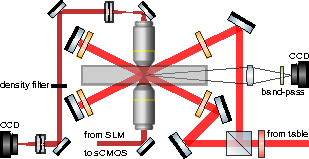
\includegraphics[width=0.85\textwidth]{figures/MOTsideview.pdf}
    \caption{Side view on the glass cell, showing vertical MOT beams under a 60 degree angle, as well as the two microscope objectives. 
    The side view MOT camera is shown as well.}
    \label{fig:GlassCellSide}
\end{figure}


\section{Characterizing the MOT}\label{sec:MOTresult}

To image the MOT we position a CCD camera\footnote{UEye UI-2230SE} looking at the MOT from the side, through the 22 by 22 mm inner dimension window at the end of the glass cell (see \cref{fig:GlassCellSide}).
It is positioned on an $X,Y,Z$ translation stage.
It has a magnification of $0.5$ using a $100$ mm focusing lens and furthermore has a 780 nm band-pass filter. 

A picture showing the laser-induced fluorescence from the MOT as imaged on the CCD camera on the side is shown in \cref{fig:LiF}.
A Gaussian fit of the spatial profile in $x$ and $y$-directions is shown in \cref{fig:LiF}.
The $1/e$ decay radius for both Gaussian fits $\sigma$ is $\sim 0.13$ mm. 
This should be sufficiently large to efficiently load an array of optical tweezers, which will be limited in size by the field of view of the microscope objective. 
Apart from the anti-Helmholtz coils, the coil design also features compensation coils in a nearly Helmholtz configuration that can be used to move the MOT in 3D space. 
The compensation coils are not perfectly Helmholtz because of limitations in space around the glass cell.
The coils not being perfectly Helmholtz might lead to a magnetic field gradient that might not be fully linear, an effect that is negligible over the dimensions of the MOT, which is tiny compared to the radii of the coils. 

When moving the MOT with the compensation coils, we see the MOT changing shape. 
A possible explanation is the unbalance in the vertical MOT beams: as a result of the rather large angle the vertical MOT beams make with the glass cell to make room for the microscope objectives, there is significant loss of power in the retro-reflected beam, which has to pass the glass cell twice. 
Because of this unbalance, the MOT probably does not sit near the zero of the magnetic field.
We think that as long as the MOT is big enough to fully overlap with the tweezer array, its exact shape should not be too important.


\begin{figure}
    \centering
    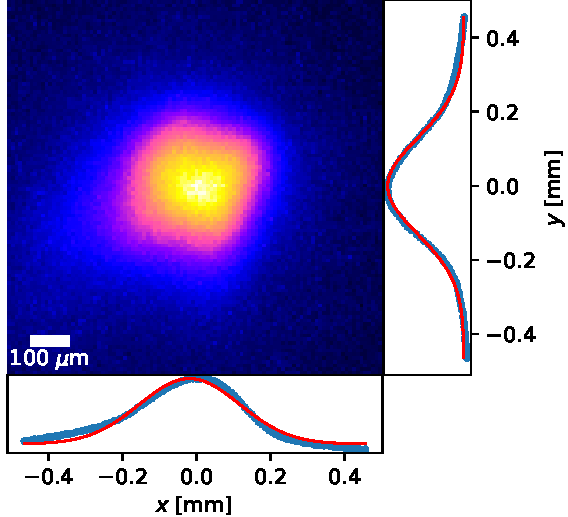
\includegraphics[width=0.55\textwidth]{figures/FluoresenceAndFits.pdf}
    \caption{A picture of laser-induced fluorescence from the magneto-optical trap as imaged onto the side camera. 
    The colors denote the relative intensity.
    Also, a Gaussian fit is shown in the $x$ and $y$-directions.}
    \label{fig:LiF}
\end{figure}

We estimate the number of captured atoms in the MOT by summing the number of counts on our side camera in a region of interest around our MOT over the pixels $j$ as $\sum_j p_j$.
A background is obtained by performing the same sum, but without magnetic field coils on and is subtracted from the result. 
We use an exposure time $\tau_s$, which varied but was typically $10$ ms, camera gain $G = 1$ and sensitivity $C$.
The camera sensitivity constant $C$ for this particular sensor at this wavelength was found to be $\sim 6 \cdot 10^3$ photons per count and was calibrated using a variety of ND filters and a laser at 780 nm of known intensity. The total number of atoms $N$ captured by our MOT is now
 
 \begin{equation}\label{eq:AtomNumber}
     N = \left( \frac{2}{\gamma\beta}\right)
     \left(\frac{4\pi l^2}{R^2}\right)
     \sum_j \frac{p_j}{\tau_s G C}.
 \end{equation}
In \cref{eq:AtomNumber} $\gamma = 2\pi \cdot 6.0$ MHz is the linewidth of the $D_2$ transition of Rb-85, $\beta \sim 0.6$ is a parameter taking into account photon loss of the glass cell and band-pass filter, $l = 20$ cm is the distance from the MOT to the collection lens and $R = 25$ mm is its radius. 
An additional factor of 2 comes in to account for the atoms occupying the excited state half of the time on average. 
We typically find a an atom number $\sim 10^5$.
This is a relatively small number of atoms for a Rb magneto-optical trap.
Possibly, this is again due to the unbalanced power in the angled beams. In a next iteration of this Rb machine or a Sr equivalent, it would be useful to have 6 independent laser beams instead of 3 retro-reflected ones, though this comes at a cost of requiring more power. 
If desired, the number could be more accurately estimated using absorption spectroscopy.
From the atom number $N$, we can estimate the peak atom density in the MOT $n_0$ as \cite{Townsend1995}

\begin{equation}
    n_0 = \frac{N}{(2\pi)^{3/2}\sigma^3}.
\end{equation}
This yields $n_0 \sim 10^9$ cm\textsuperscript{-3}, which is sufficiently high to load a microscopic optical dipole trap comparing to the values mentioned in \cite{Schlosser2002} and comparing to our collaborators working with Sr atoms.


\section{Imaging Tweezer Arrays}\label{sec:Tweezers}

We will now explain how we use the optical tweezer setup of \cref{ch:tweezer,ch:arrays} to trap neutral atoms. 
The optical setup used for the optical tweezer array was already introduced in \cref{fig:TiSandSLMsetup,fig:SLMbeampath}b.
The implementation of this setup in the machine is shown in \cref{fig:GlassCellTop}.
Using two sets of relay-mirrors, the beam from the \ac{SLM} is steered to the mirror sending the beam in vertical direction to the microscope objective, see \cref{fig:GlassCellSide}. 
In reality, from the top view in \cref{fig:GlassCellTop} the horizontal MOT beam and tweezer beam overlap with each other, therefore the tweezer beam is shown under a slight angle here.
A polarizing beam splitter cube is added which can be used to add additional laser beams to send into the objective, e.g. Rydberg lasers or laser beams for re-arrangement of the optical tweezer array. 
At the moment, this cube is unused, but we added it because it will change the optical path length of the SLM-objective path.

The microscope objective is again positioned on the same 5-axis piezo stage as used in \cref{fig:TiSandSLMsetup,fig:ZScanSetup} using a custom aluminum holder.
To allow for arbitrary positioning of the stage with respect to the glass cell, it is not mounted directly into the vertical breadboard but in a set of base-plates that in turn screw into the table.
The holder is shown in \cref{fig:Coils}.
\begin{figure}
	\begin{subfigure}{.49\linewidth}
		\flushleft
		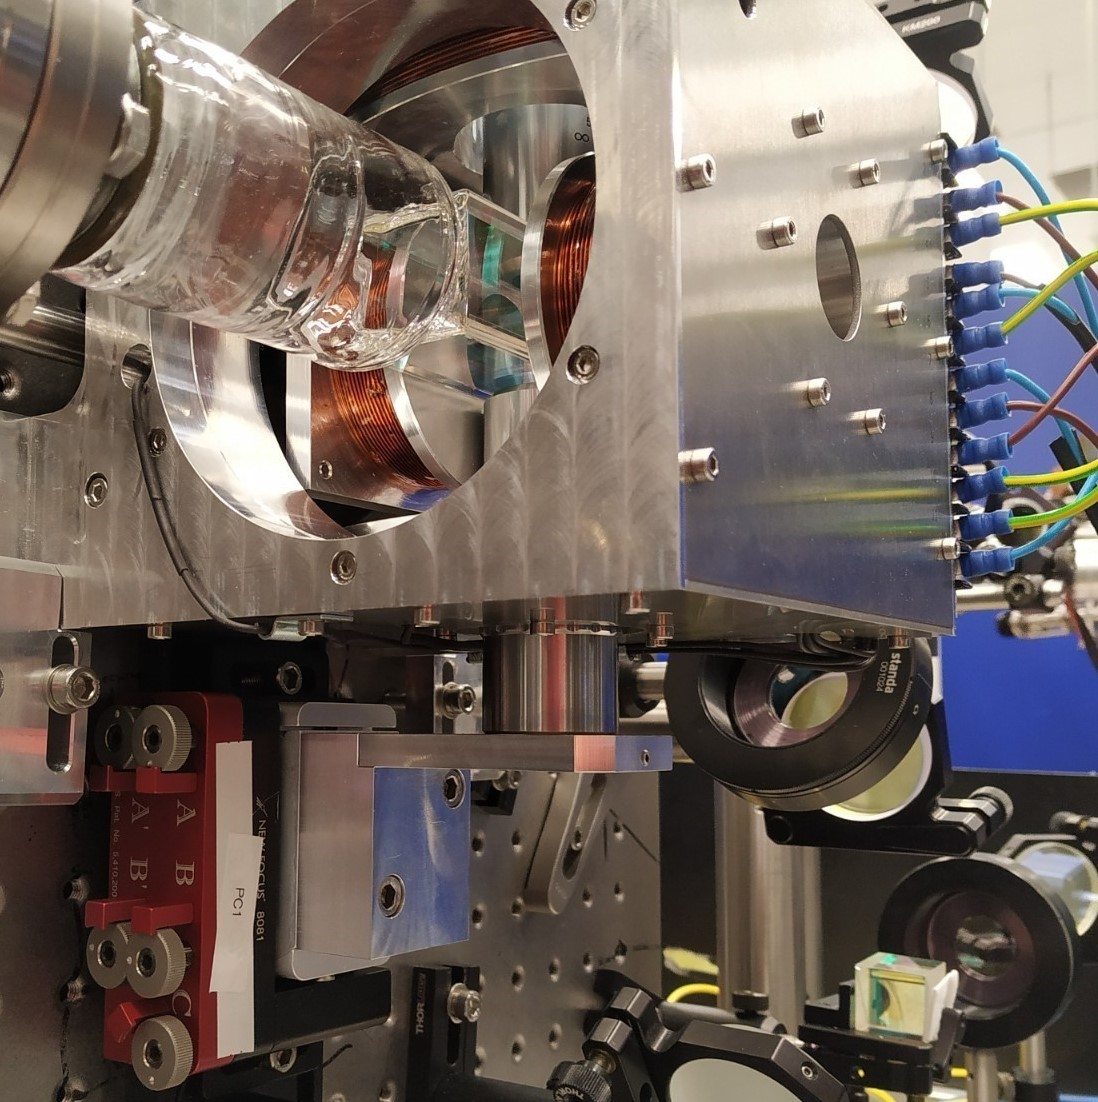
\includegraphics[height=7.6cm]{figures/CoilsCropped.jpg}
		\caption{}
		\label{fig:Coils1}
	\end{subfigure}
	\hfill
	\begin{subfigure}{.49\linewidth}
		\flushright
		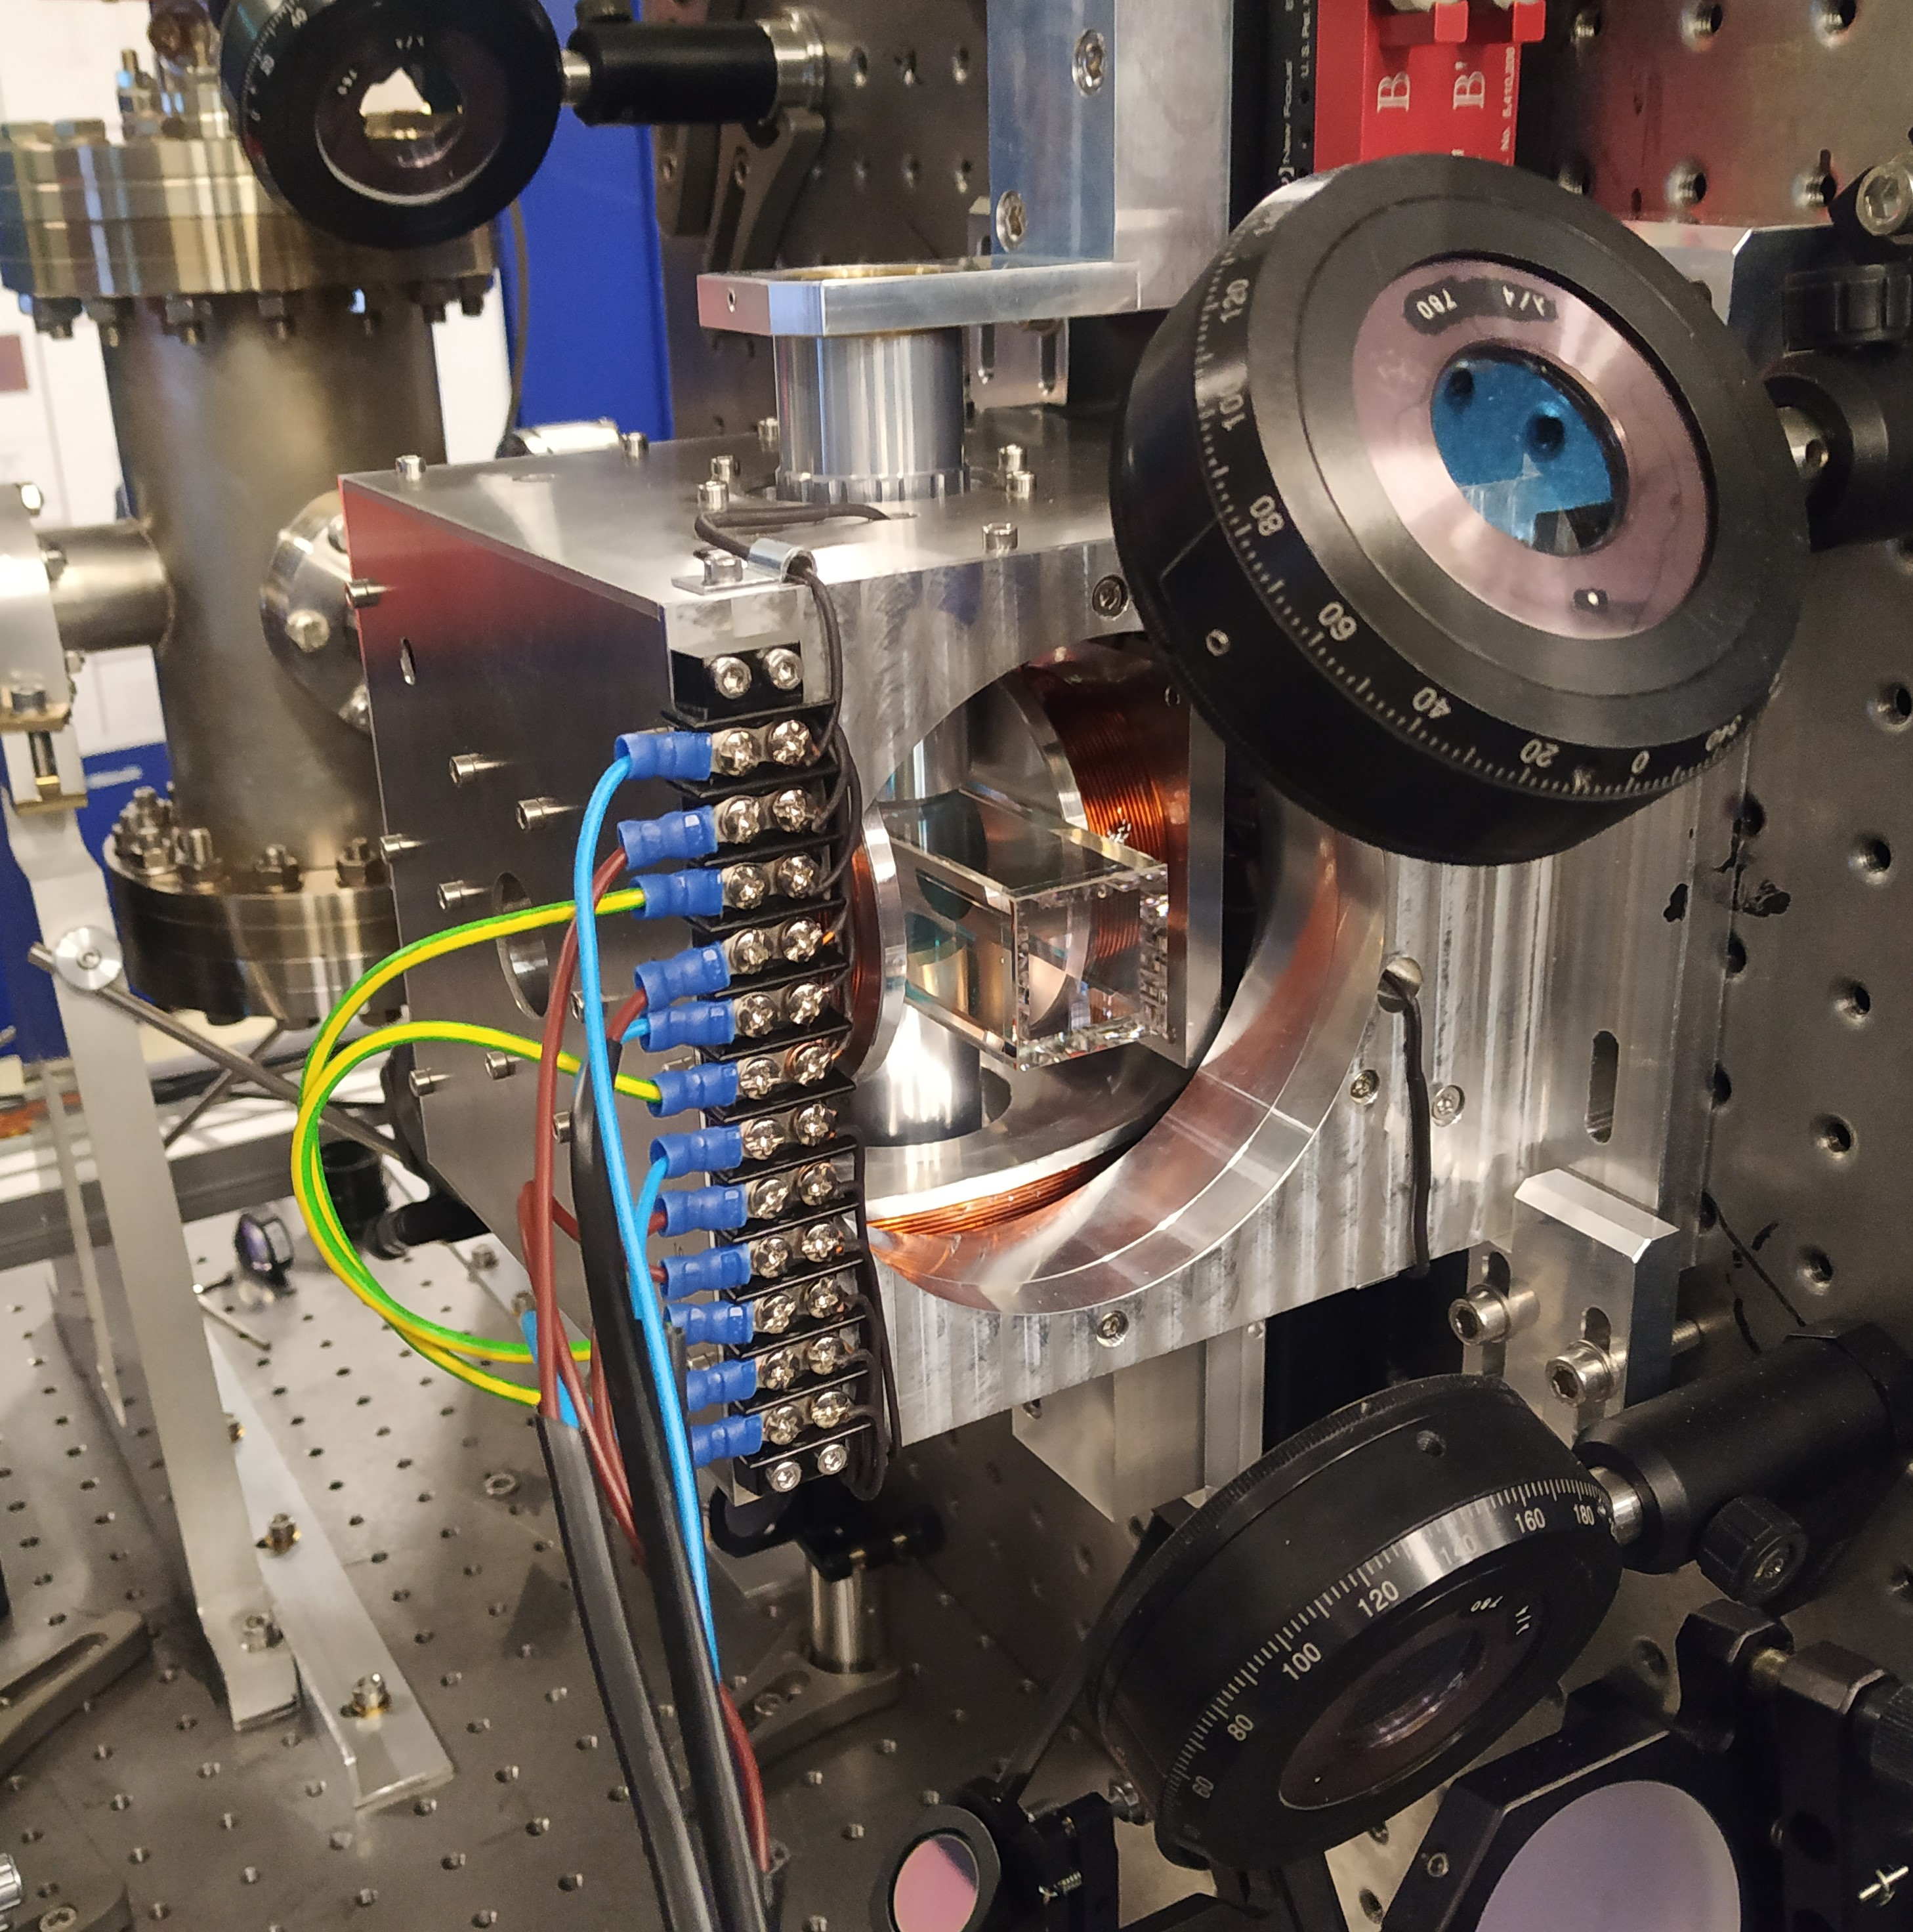
\includegraphics[height=7.6cm]{figures/CoilsCropped2.jpg}
		\caption{}
		\label{fig:Coils2}
	\end{subfigure}
	\caption{
	\textsf{\textbf{a)}} Housing for the magnetic field coils. 
	The glass cell slides into the magnetic field coils enclosure.
    The microscope objectives are positioned on 5-axis piezo controlled stages using a custom aluminum mount. 
    \textsf{\textbf{b)}} Different angled picture, showing the vacuum vessel in the background as well. 
    The large holes in the enclosure for the coils is for the angled MOT beams.
    }
    \label{fig:Coils}
\end{figure}
To load the tweezer array with the with atoms it is overlapped with the magneto-optical trap. 
The most straightforward method is to move the MOT in 3D-space using additional bias coils.
The field along the direction of the Anti-Helmholtz coils is adjusted by superimposing a bias current, which equates to running the Anti-Helmholtz coils with unequal current. 
Typically we run the Anti-Helmholtz coils with $1.36$A and $1.4$A, while the compensation coils are run with $0.5$ and $0.2$A.
The power supply used to drive the coils\footnote{KORAD KC3405 programmable DC power supply} as well as the \ac{AOM}s are controlled by a custom Python control program written by Deon Janse van Rensburg, with a graphical user interface in \textit{PyQt}.

We found moving the MOT to work very nicely over a range of $\sim 1$ cm, which is more than plenty in overlapping with the \ac{ODT}.
To verify the overlap, we use an identical Mitutoyo objective above the glass cell.
This objective is brought in focus with the tweezer light, and subsequently the MOT is moved until we see the MOT through both objectives. 
This ensures that the MOT is overlapped in 3D space with the tweezers .
The image from the top objective is focused onto another UEye UI-2230SE \ac{CCD}, which has its cover glass removed to avoid aberration and interference effects. 




\subsection{Direct Imaging: Tweezer Arrays}\label{sec:TweezerImaging}

When imaging our tweezer array, we can look directly at the light distribution itself, as seen through the top objective imaged onto a CCD (direct imaging).
This is not only useful to check for overlap with the MOT, it also allows to check whether the dipole potentials remain aberration free during the experiment \cite{Baumgaertner2017}.
Lastly, directly measuring the light potentials allows for dynamic adaption of the weight factors in the \ac{GSW} algorithm to increase the uniformity of the array \cite{Nogrette2014}.

Contrary to the method in \cref{ch:tweezer}, loss of information about the tweezer array is unavoidable because the imaging resolution will be similar to the feature size one is looking at.
To directly see our dipole potentials, we use a second, identical long-working distance positioned at the opposite end of the glass cell, because the glass cell outer thickness is 30 mm. 
The microscope objective has a working distance when imaging through 3.5 mm N-BK7 glass of 15.08 mm, but we know that the glass cell has 4 mm thick quartz glass.
Consequently, there is a slight increase in the optical thickness of $n d_{\text{ex}}$ where $d_{\text{ex}}$ is the physical thickness of the extra glass.
As a result, the paraxial rays focus a distance $d_{\text{ex}}(1-1/n)$ further.
Thus, in conjunction with this glass thickness $d_{ex} = 0.5/n$ mm we estimate the new working distance to be $15.08 + d_{\text{ex}}(1-1/n) \approx 15.18$ mm.
Consequently, it should be possible to get a second objective in infinity conjugate configuration, but this requires positioning the objective less than $0.2$ mm from to the glass cell.

Still, we did not manage to get a collimated beam out of the top microscope objective, even when bringing it so close to the glass cell it is almost touching. 
A shown in \cref{fig:GlassCellSide} the beam coming out of the objective forms a focus.
We use an achromatic lens to collimate this beam agin.
The objective is designed for infinite conjugate operation and will thus contain aberration. 
For now, it is not a problem the image on the camera from the top objective is slightly abberated, but for the next iteration of the machine we ordered a new glass cell from Japan Cell with 25 mm outer thickness, making it easier to get the objectives in focus with each other while also having infinite conjugate configuration.

\subsection{Fluorescence Imaging: Tweezer Arrays}


To verify atoms are trapped in the tweezers, we have to induce scattering using near-resonant light (probing). 
While the MOT beams we already have could be used for this, the vertical MOT beams enter the cell under a 60 degree angle.
We worried this would cause too much background light in the vacuum chamber, which will enter the objective as well. 
Therefore, we used a separate beam path, the probe beam as shown in \cref{fig:RbLaserSetup}, which we only direct in the horizontal beam path using the $\lambdaup/2$ plate in \cref{fig:GlassCellTop}.
This is the same beam path as the repump EOM is positioned in, but because the the polarization is orthogonal to the horizontal MOT beam, the EOM will leave the probe light unaffected. 
We typically run the probe with a blue detuning of $\delta \sim +3\gamma$: the atomic transition is Stark shifted to the blue (see \cref{fig:DipoleForce}) and intensity $I = 0.5 I_{\text{sat}}$, which for our beam diameters comes down to $\sim0.$5 mW per beam\footnote{The saturation intensity of the Rb-85 $D_2$-transition is approximately 1.6 mW/cm\textsuperscript{2}}. 

\subsubsection*{Collecting Light}

Because fluorescence from atoms in tweezers is typically fairly weak, we maximize the amount of scattered photons that we can actually collect. 
The fraction $\eta$ of fluorescence that can be captured by our imaging system is the fraction of the collection solid angle $\Omega$ over the full solid sphere $4\pi$

\begin{equation}\label{eq:Collection}
    \eta = \frac{\Omega}{4\pi} = 
    \frac{1}{2}\left(1-\sqrt{1-\frac{\text{NA}^2}{n^2}}\right).
\end{equation}
For $\text{NA}=0.5$ and $n=1$ we find $\eta =0.067$. 
We collect the laser-induced fluorescence using the same microscope objective as used for producing the tweezer, separating it from the tweezer beam using a \ac{DM}\footnote{Thorlabs DMLP805, 1 inch}.
This is shown in \cref{fig:GlassCellTop}.
This dichroic mirror has a 805 cut-off, which is why 820 nm was chosen for the dipole traps.
The top objective could also be used to collect fluorescence, but it will contain aberration as it cannot be brought close enough. 
Additionally, we found it was non-trivial to fully filter out the tweezer light, which is all collected by the top objective as it is positioned in focus with the bottom objective. 

The fluorescence is steered onto the Andor Zyla 5.5 sCMOS camera chip covered by a 780 band-pass filter, see \cref{fig:GlassCellTop,fig:GlassCellSide}.
The pixel size is 6.5 $\mu$m, or 19.5 $\mu$m using $3\times3$ pixel binning. 
It is focused onto the chip using a $f= 55$ mm lens\footnote{Nikon Micro-NIKKOR 55 mm f/2.8}.
Using \cref{eq:InfinityMagnification} this comes down to a magnification factor of $13.75$.
We assume our spots are $0.8$ $\mu$m in $1/e^2$ radius (\cref{sec:TweezerRadial}).
After convolution with the imaging optics this comes down to roughly $1.1$ $\mu$m.
With the $13.75$ magnification, we estimate $3\times3$ pixel binning would probably work best: imaging a single spot on a single binned pixel should maximize the signal to noise ratio. 
If the tweezer spot is not aligned perfectly with a $3\times3$ binned pixel, it is possible it will light up $1\times2$ or $2\times2$ (binned) pixels as well.
We focus the sCMOS camera by adjusting the $f=55$ mm field lens.
We do not have a feature we can focus onto, but we know we should be focused at infinity to be in focus with our tweezer array. 
We ensure we focus at infinity by shining a laser source collimated by a fiber outcoupler directly onto our camera, adjusting the focus until the parallel beam is imaged onto the chip as a diffraction-limited spot. 

\subsubsection*{Experimental Sequence}

Our experimental sequence for recording fluorescence from atoms in tweezers is shown in \cref{fig:Sequence}.
After letting the MOT build up for about 400 ms, we overlap the tweezer with it for about 150 ms.
Turning the tweezer on and off is controlled by a mechanical shutter positioned on the \ac{Ti:S} laser table, in order to avoid the MOT laser losing lock from the shutter.
The delay of the mechanical shutter is in the of order of a couple ms. 
During imaging, the MOT beams are turned off.
We do this by using their \ac{AOM}s, which can be turned off in a matter of micro seconds. 
The imaging consists of triggering the probe beam as well as triggering the sCMOS camera at the same time. 
For the images shown here, we used a 10 ms delay after turning off the MOT beams to the start of triggering the sCMOS camera. 
The triggering sequences are fed to the hardware using a programmable pattern generator custom built in our group. 
The imaging sequence is shown in \cref{fig:Sequence}.
\begin{figure}
    \centering
    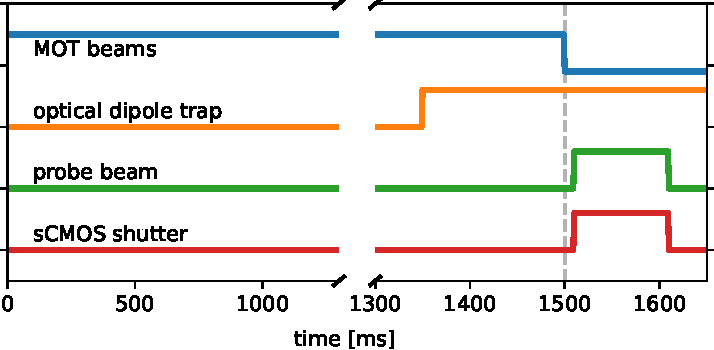
\includegraphics[width=0.73\textwidth]{figures/Sequence.pdf}
    \caption{Experimental sequence used to record laser-induced fluorescence from atoms trapped in an array of optical tweezers.
    The probe and sCMOS are turned on shortly after turning off the MOT beams. }
    \label{fig:Sequence}
\end{figure}
For now, we do not turn off the magnetic field of the MOT.
The currents producing the field can be shut off, but the speed at which this can be done is limited by Eddy currents in the aluminum enclosure of the coils. 
Rik van Herk measured a $1/e$ decay time of 8 ms.
If we switch off the field prior to imaging, we can perform spectroscopy and measure the AC stark shift as a function of probe detuning. 
With the fields on however, there will also be Zeeman energy shifts in the array according to \cref{eq:DetuningFull}. 

\subsubsection*{Images}

Using the experimental sequence in \cref{fig:Sequence} we obtain fluorescence as shown in \cref{fig:fluorescence} for $2\times2$ and $2\times3$ arrays using the SLM respectively.
For better visibility, we increased the spacing between the spots to $\sim 12$ $\mu$m.
We also performed exactly the same experimental sequence, but without ever turning on the dipole trap laser. 
The latter should only yield background as a result of remaining atoms from the expanding MOT or scattered photons from probe beam.
We subtract the latter result from the image where we do turn on the tweezer light.
The difference will be the fluorescence from atoms trapped in the tweezer array. 
This procedure was averaged a number of times as the signal to noise ratio was too low when not averaging, yielding for 50 averages the arrays in \cref{fig:fluorescence}.
To verify that this is not a reflection from the tweezer light itself, we also re-ran the sequence but with the MOT repump light off.
In this case, we never build a MOT and we should not load the tweezers, which indeed only yielded noise.
At the moment, we cannot do a larger number of spots because of limits in laser power.
We tried lowering the trap depth of the optical tweezers, which would lower the amount of power needed per trap, but we noticed the quality of the signal significantly deteriorated as a result. 


\begin{figure}
    \centering
	\begin{subfigure}{.49\linewidth}
		\centering
		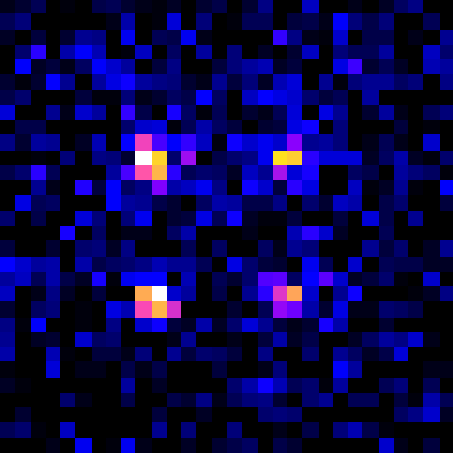
\includegraphics[height=5cm]{figures/2x2fluorescence.pdf}
		\caption{}
		\label{fig:fluor2x2}
	\end{subfigure}
	\hfill
	\begin{subfigure}{.49\linewidth}
		\centering
		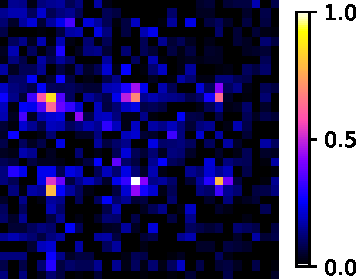
\includegraphics[height=5cm]{figures/2x3fluorescence.pdf}
		\caption{}
		\label{fig:fluor2x3}
	\end{subfigure}
	\caption{
	Fluorescence imaged onto the sCMOS camera when \textsf{\textbf{a)}} applying a $2\times2$ array pattern to the SLM as well as \textsf{\textbf{b)}} a $2\times 3$ array.
	Averaged over 50 runs.
    }
    \label{fig:fluorescence}
\end{figure}
\Cref{fig:fluorescence} would suggest the signal to noise ratio is low. 
This is confirmed by performing different number of averages.
In \cref{fig:Averaging} we show the same result averaged 10, 30 and 50 times. 
The signal to noise increases for higher number of averages.
One cause could be that we are loading a very low number of atoms in our tweezer array, for instance less than 0.5 on average per tweezer site as predicted by the collisional blockade mechanism (\cref{sec:LoadingAtoms}).
We think this is unlikely however: while estimating the loading rate $R$ is non-trivial, we can use a simple model to see what this loading rate $R$ depends on. 
For low loading rates, the dipole trap loading can be described as \cite{Kuppens2000}

\begin{equation}\label{eq:Loading}
    R \propto n_0 \bar{v} A\propto n_0 T^{1/2} w_0^2.
\end{equation}
Here, $A$ is the area of the dipole trap as seen by the atom approaching with average velocity $\bar{v}$. 
In our case $A \propto w_0^2$.
The average velocity is proportional to the temperature as $\bar{v}\propto T^{1/2}$.
Because we have similar cold atom densities $n_0$ to other groups, and our temperature of $220$ $\mu$K is relatively hot compared to other groups (which means slightly higher loading according to \cref{eq:Loading}), we find it unlikely our loading rate would be very low. 
Rather, we think it is a camera issue. 
We noticed the camera does not fully clear its charge prior to imaging, which would show up in the image as noise. 
Additionally, our camera shows a high amount of noise (dark current or clock induced charge, as well as readout noise) compared to the detected signal.
Finally it has a low quantum efficiency at 780 nm, lowering our detection fidelity. 

The issue of the charge not clearing could be solved by installing a mechanical shutter in front of the sCMOS camera, blocking any MOT light prior to imaging from hitting the chip. 
This would have to be quite a large shutter.
Alternatively, the light could be focused to an smaller spot using a beam expander, shuttering in the intermediary focus point of the telescope. 
The latter approach has the advantage that it also allows to do spatial filtering: which is to filter out light not originating from the focus of the tweezer. 
 

\begin{figure}
    \centering
	\begin{subfigure}{.31\linewidth}
		\centering
		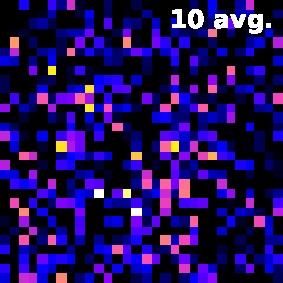
\includegraphics[height=4.5cm]{figures/10avg.pdf}
		\caption{}
		\label{fig:10avg}
	\end{subfigure}
	\hfill
	\begin{subfigure}{.31\linewidth}
		\centering
		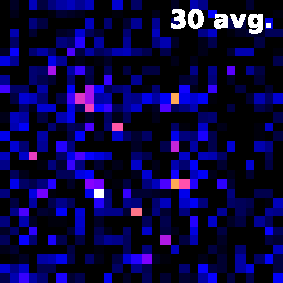
\includegraphics[height=4.5cm]{figures/30avg.pdf}
		\caption{}
		\label{fig:30avg}
	\end{subfigure}
	\hfill
	\begin{subfigure}{.33\linewidth}
		\centering
		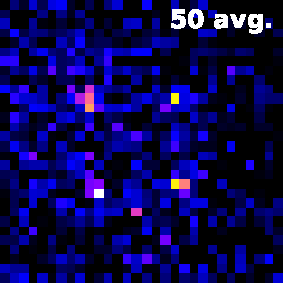
\includegraphics[height=4.5cm]{figures/50avg.pdf}
		\caption{}
		\label{fig:50avg}
	\end{subfigure}
	\caption{Evolution of the signal to noise with the number of averages for a $2\times 2$ array for \textsf{\textbf{a)}} 10 \textsf{\textbf{b)}} 30 and \textsf{\textbf{c)}} 50 averages.
    }
    \label{fig:Averaging}
\end{figure}





